\chapter{Simulations of a Population Model Which Incorporates Density-Dependent Somatic Growth}

\section{A Density-Dependent Finite-Dimensional Model} \label{section:finitedim}

The size distribution of ecological populations sometimes becomes skewed towards smaller members, which can happen when a species is invasive or when the biomass is large. The papers \cite{Chizinski2010, Ylikarjula1999} suggest that in these situations, increased competition for food could explain why individuals do not reach larger sizes over time. The authors of these papers were interested in \emph{stunting}, which happens when individuals are smaller than expected for their age. Hence, the model in \cite{Chizinski2010, Ylikarjula1999} keeps track of the age of individuals, and also their size. This combination of age- and size-structure is hard to analyze mathematically, so \cite{Callahan2019} gave a simplified model which incorporates density-dependent somatic growth as in \cite{Chizinski2010, Ylikarjula1999}, but which does not keep track of age-cohorts. The model in \cite{Callahan2019} is a nonlinear matrix model of the form
\begin{align}
	n_{t+1} = A_{w_t} n_t, \quad t \in \N \cup \{0\}, \label{eqn:matrixsystem}
\end{align}
where $n_t \in \R^{j+1}$ is a population vector. The matrix $A_{w_t}$ is given by
\[A_{w_t}:= \begin{pmatrix}
0 & f_1 & f_2 & f_3 & \cdots & f_{j-2} & f_{j-1} & f_j \\
s_0 & s_1(1-w_t) & 0 & 0 & \cdots & 0 & 0 & 0 \\
0 & s_1 w_t & s_2(1 - w_t) & 0 & \cdots & 0 & 0 & 0 \\
\vdots & \vdots & \vdots & \vdots & \ddots & \vdots & \vdots & \vdots \\
0 & 0 & 0 & 0 &\cdots & s_{j-2} w_t & s_{j-1} (1- w_t) & 0 \\
0 & 0 & 0 & 0 & \cdots & 0 & s_{j-1} w_t & s_j
\end{pmatrix},\]
where the $f_i$ and $s_i$ values are fecundity and survival rates, respectively, and $0 \leq i \leq j$ enumerate increasing size classes. Additionally, the authors of \cite{Callahan2019} assume that $f_i>0$ for each $i$, and that $s_i$, $f_i$ are non-decreasing in $i$. This is a reasonable assumption, because larger individuals are often more likely to survive than their smaller conspecifics, and larger  individuals often have more offspring (i.e., fish are able to carry more eggs). The value $w_t$ is the probability of a stage $i$ individual growing to the stage $i+1$ in one time step (without considering mortality). This probability is a function of the total biomass of the population at time $t$:
\[w_t = w(B_t),\]
where $w: [0,\infty) \to (0,1]$ is a differentiable and strictly decreasing function, with $w(0) = 1$, $\lim_{y \to \infty} w(y) = 0$. The biomass at time $t$ is given by
\begin{align}
	B_t := \alpha \sum_{i = 0}^{n+1} L_i^3 n_t^i, \label{eqn:matrixbiomass}
\end{align}
where $n_t^i$ is the $i$th entry of the population vector $n_t$, and $L_i$ is the assumed length of individuals in that class.

The primary result of \cite{Callahan2019} is the following (which is Theorem 1 in original paper):

\begin{theorem} \label{thm:finitedimtheorem}
	Assume that $L_i$, $s_i$, and $w(\cdot)$ satisfy the properties given above. Then the system
	\begin{align}
		n_{t + 1} = A_{w_t} n_t, \quad w_t = w(B_t) \label{eqn:system}
	\end{align}
	satisfies the following:
	\begin{enumerate}
		\item for $0 \leq v \leq w \leq 1$, $r(A_v) \leq r(A_w)$;
		\item if $r(A_1) < 1$, then the zero-population $n_0 \equiv 0$ is globally asymptotically stable;
		\item if $r(A_0) >1$, then $\lim_{t \to \infty} ||n_t|| = \infty$ for all nonzero nonnegative initial states $n_0$;
		\item if $r(A_0) < 1 < r(A_1)$, then the system \eqref{eqn:system} is bounded and has a unique nonzero equilibrium $n^*$, and for every nonnegative initial population $n_0$, the biomass converges to the equilibrium biomass:
		\[\lim_{t \to \infty} B_t = B^*,\]
		where $B^*$ is the biomass of the population $n^*$.
	\end{enumerate}
\end{theorem}
We note that in the original paper, this theorem also has results about the persistence of the population, but for clarity we omit these results, as they were not important in motivating our work with the nonlinear IPM.

The statement of Theorem \ref{thm:finitedimtheorem} shows that the Perron-Frobenius theory for matrices is critical in understanding the system \eqref{eqn:system}, since the results depend on knowledge of the spectral radii of $r(A_0)$ and $r(A_1)$, where $0$ and $1$ are the extreme values of $w_t$. The fact that $r(A_0)$ and $r(A_1)$ are eigenvalues of the matrices $A_0$, $A_1$, respectively, is guaranteed by the classical Perron-Frobenius theorem for matrices. Note that in the matrix $A_{w_t}$ above, individuals cannot shrink in size between time steps; a nonlinear IPM which incorporates density-dependent growth will thus have an unbounded growth kernel for any fixed biomass value, and the associated linear operator will be non-compact. We expect the main result of Section \ref{section:mainresults} to be useful in proving results about a nonlinear IPM model analogous to \eqref{eqn:system}, which we describe in the next section. 

\section{A Density-Dependent IPM} \label{section:ddipm}

We used the IPM operator $T:L^1 \to L^1$ given in \cite{Vindenes2014} as the basis for a nonlinear operator $T_{w_t}:L^1 \to L^1$ which incorporates density-dependent somatic growth (see \eqref{eqn:ddkernel} below). In this section, we study the system
\begin{align}
	\varphi_{t+1} := T_{w_t} \varphi_t, \quad w_t:=w(B_t), \label{eqn:ipmsystem}
\end{align}
again where $w:[0,\infty) \to (0,1]$ is a differentiable, strictly decreasing function such that $w(0) = 1$, and $\lim_{y \to \infty} w(y) = 0$. In \eqref{eqn:ipmsystem}, the value $B_t$ is the biomass of the population vector $\varphi_t$, which we compute as
\begin{align}
	B_t:= \alpha \int_L^U x^\beta \varphi_t(x) \, dx, \label{eqn:ipmbiomass}
\end{align}
analogously to \eqref{eqn:matrixbiomass}. In both definitions \eqref{eqn:matrixbiomass} and \eqref{eqn:ipmbiomass}, the parameter $\alpha$ is the mass-length coefficient of the modeled population. Finally, the nonlinear operator $T_{w_t}:L^1 \to L^1$ is the integral operator with kernel
\begin{align}
	k(y, x, w_t) := s(x)g(y, x, w_t) + b(y)f(x), \label{eqn:ddkernel}
\end{align}
where the survival function $s(x)$, offspring distribution $b(y)$, fecundity $f(x)$ are given in \cite{Vindenes2014}.  We incorporated density-dependent growth into their model by replacing the mean growth increment $(m(x) - x)$ with $w_t(m(x) - x)$. Hence, when the population biomass increases, $w_t$ will be decrease and so will the mean growth increment. Specifically, we used the mean growth $m(x)$, standard deviation of growth $\sigma(x)$, and lognormal parameter conversions $\mu(x)$ and $v(x)$ also used in \cite{Vindenes2014} to define
\begin{align}
	g(y, x, w_t) := \left\{ \begin{array}{lc} \frac{\Gamma(y, x, w_t)}{\int_x^U \Gamma(y, x, w_t) \, dy}, & y > x, \\ 0, & y \leq x \end{array} \right. ,
\end{align}
where
\begin{align}
	\Gamma(y, x, w_t) &:= \frac{1}{\sqrt{2 \pi}(y - x) v_{w_t}(x)} \exp \left( - \frac{(\ln(y - x) - \mu_{w_t}(x))^2}{2 v_{w_t}(x)} \right), \label{eqn:gammadef}\\
	\mu_{w_t}(x) &:= \log \left( \frac{((w_t(m(x)-x))^2}{\sqrt{((w_t(m(x) - x))^2 + \sigma(x)^2}}\right), \label{eqn:mudef}\\
	v_{w_t}(x) &:= \log \left( 1 + \frac{\sigma(x)^2}{(w_t(m(x)-x))^2}\right).	\label{eqn:vdef}
\end{align}
We incorporated the same functional response $w(y)$ used in \cite{Callahan2019}, namely 
\begin{align}
	w(y) := \frac{1}{1 + c y}, \label{eqn:wdef}
\end{align}
where $c$ is a parameter that depends on the population. However, since equations \eqref{eqn:mudef} and \eqref{eqn:vdef} are both undefined when $w_t = 0$, we have to bound $w_t$ away from zero in order to avoid division by zero on the computer. Even though $w(y)>0$ for all $y$, in some simulations the population biomass $B$ gets so large that computers evaluate $w(B)=0$. Hence, we used the function
\[w_t := \max \left\{\frac{1}{1 + c B_t}, 0.001 \right\}\]
where $B_t$ is defined in \ref{eqn:ipmbiomass}. 

Note that in the matrix system \eqref{eqn:matrixsystem}, $w_t$ is the probability that an individual in size class $i$ will grow to size $i+1$. However, in the IPM system \eqref{eqn:ipmsystem}, $w_t$ must have a different interpretation, since in this case the size stages are continuous. Using 

The definitions \eqref{eqn:linearmudef} and \eqref{eqn:linearvdef} indicate the conceptual difference between the role of $w_t$ in the matrix system \eqref{eqn:matrixsystem} and the IPM system \eqref{eqn:ipmsystem}: in the former, $w_t$ is the probability that an individual in size class $i$ grows to size class $i + 1$ in a single time step (ignoring mortality), and in the latter, $w_t$ represents a scale factor that reduces the expected growth increment $(m(x) - x)$ of an individual of size $x$ as the total biomass increases.

The expressions \eqref{eqn:gammadef} - \eqref{eqn:vdef} look complex, so to clarify the effect of scaling the quantity $(m(x) - x)$ by $w_t$, we include Figure \ref{fig:nonlinear_comparison}:

\begin{figure}[H]
	\centering
	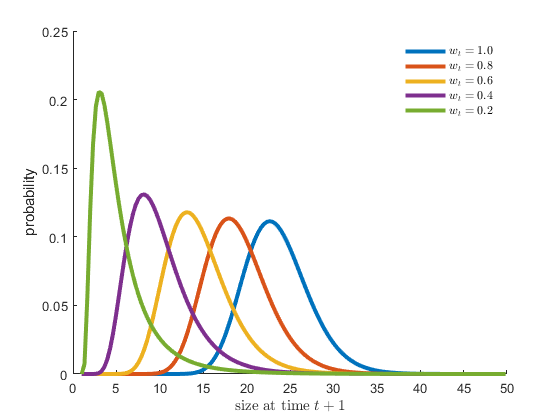
\includegraphics[width=0.6\linewidth]{Images/nonlinear_comparison}
	\caption{Plots of $g(y, x, w_t)$ for $x = 1$ and various values of $w_t$}
	\label{fig:nonlinear_comparison}
\end{figure}

Since smaller values of $w_t$ correspond to higher biomass, this plot indicates that a size $x=1$ individual is likely to grow less when total population biomass is high. The value $x=1$ is not special; other values of $x$ yield similar plots.

\begin{figure}
	
\end{figure}

\section{Simulation Results}

In the following subsections, we give simulation results based on the system \eqref{eqn:ipmsystem}, but with some caveats. We used MATLAB to generate a matrix at each time step which sampled the kernel of $T_{w_t}$ using a mesh of 300 equally spaced points on the $x-$ and $y-$axes; however, Corollary \ref{th:corollarytonotweaklycompact} says that $T_{w_t}$ is not compact for any value of $w_t \in (0,1]$, and hence cannot be approximated by matrices. Because of this, we do not claim that our simulations reflect the true dynamics of the infinite-dimensional system. Instead, one could think of the nonlinear IPM as a tool to generate a finite-dimensional system with as many size classes as mesh points as one chooses, and which allows for more growth options than the matrix $A_{w_t}$ in \cite{Callahan2019}.

With that said, we make one more assumption on the IPM model in three of the following subsections, namely that individuals all have the same survival rate, regardless of size. This is consistent with our assumption in Section \ref{section:operatordef}, in which we assumed $s(x)$ was increasing, but not necessarily strictly increasing. For constant survival, the simulations suggest that a result akin to Theorem \ref{thm:finitedimtheorem} may hold for the nonlinear IPM system. In subsections \ref{subsec:0.05f(x)}, \ref{subsec:f(x)}, and \ref{subsec:1000f(x)}, we assume that the survival probability for all sizes is $0.68$, which is the maximum survival rate given in \cite{Vindenes2014}. 

We decided to assume constant survival because the long-term behavior of the IPM system \eqref{eqn:ipmsystem} is unclear for the sigmoid-shaped survival function $s(x)$ given in \cite{Vindenes2014}. In this case, the survival of offspring is extremely low, and the resulting populations grow very slowly. Hence, it is hard to tell from plots what the population is doing in the long-run. With this more realistic survival function, the asymptotic behavior of the system is not at all clear, even after thousands of time steps. Hence, for this preliminary investigation, we will keep the survival rates for each size constant.

In the results that follow, we allowed the IPM system to evolve for 200 time steps, starting from five different initial populations $p_i = v_i/||v_1||_1$, where
\begin{align}
	v_i(x) = \begin{cases} 1, & x \in \left[L + \frac{1}{5}(U-L)(i-1), L + \frac{1}{5}(U-L)i \right] \\ 0, & \text{else} \end{cases}
\end{align}
for $i = 1, 2, 3, 4, 5$, and where $L$, $U$ are the lower- and upper-limits of $x$, respectively. These vectors give a different initial concentrations in ranges that span the whole state space $[L, U]$. Note also that $||p_i||_1 = 1$ for all $i$; we tested larger initial populations (up to 10,000 individuals), but changing the population size did not change the asymptotic behavior of the model.

In subsections \ref{subsec:0.05f(x)} - \ref{subsec:1000f(x)}, we investigated whether results like parts (2)-(4) of Theorem \ref{thm:finitedimtheorem} held. In the first simulations, we scaled the fecundity function $f(x)$ given in \cite{Vindenes2014} by 0.05, and in this case the population went extinct. Second, we left $f(x)$ unchanged, and this yielded a positive steady state population. Third, we scaled $f(x)$ by  a factor of 1000, which yielded a population going to infinity. In the respective simulations, the biomass went 0, a positive value $B^*$, and infinity. Hence, the operators $T_{w_t}$ appear to approach the linear operators $T_1$, $T_{w^*}$, or $T_{0.001}$, respectively, where
\[w^*:= \max \left\{ \frac{1}{1 + c B^*}, 0.001 \right\}.\]
Because of this, each of the normalized population vectors $p_t/||p_t||$ in Subsections \ref{subsec:0.05f(x)} - \ref{subsec:1000f(x)} approached a steady state distribution given by the leading eigenvector of the respective linear operators $T_1$, $_{w^*}$, and $T_{0.001}$. By only altering the fecundity function of the various kernels, we were able to directly compare these steady state distributions; this is because the different scaling factors on $f(x)$ disappear during  normalization, a fact guaranteed by the formula 
\[\psi = F(\lambda I - GS)^{-1}b\]
for the leading eigenvector of a the linear IPM operator (see Corollary \ref{th:existenceofevector}). Since this nonlinear IPM is a model of density-dependent somatic growth, directly comparing the steady state distributions allows us to verify that higher biomass leads to populations dominated by smaller individuals.

Before we give simulation results, we stress again that we do not know whether they accurately portray the dynamics of the infinite-dimensional system \ref{eqn:ipmsystem}. This is because for a fixed $w_t = w$, we cannot uniformly approximate the linear operator $T_w$ with matrices, since $T_w$ is not compact (see Theorem \ref{th:corollarytonotweaklycompact}. And if we cannot uniformly approximate a particular $T_{w}$, we also cannot make a claim about the asymptotic behavior of the full nonlinear system $\varphi_{t+1} = T_{w_t} \varphi_t$. Instead, we consider the following results to be for a high-dimensional matrix model, obtained by sampling the kernel \eqref{eqn:ddkernel} with $300^2$ mesh points. 

We summarize the functions and parameters we used in the following table:

\begin{table}[h!]
	\begin{center}
		\caption{Kernel functions and parameters}
		\label{tab:funcsandparams}
		\begin{tabular}{c|c|c}
			\hline
			 & \textbf{Description} & \textbf{Source}\\
			\hline \hline
			$b(y)$ & offspring distribution & \cite{Vindenes2014} \\
			$f(x)$ & fecundity & \cite{Vindenes2014} \\
			$g(y, x, 1)$ & somatic growth, no biomass & \cite{Vindenes2014} \\
			$s(x) \equiv 0.68$ & survival probability & \cite{Vindenes2014} \\
			$\alpha = 6.648 \times 10^{-6} \text{kg}/\text{cm}^3$ & conversion rate in \eqref{eqn:ipmbiomass} & \cite{Milardi2014} \\
			$\beta = 3.0217$ & power in \eqref{eqn:ipmbiomass} & \cite{Milardi2014} \\
			$c = 9.0 \times 10^{-3} \text{kg}^{-1}$ & factor in \eqref{eqn:wdef} & \cite{Chizinski2010}, converted to $\text{kg}^{-1}$ \\
			\hline
		\end{tabular}
	\end{center}
\end{table}

We note that the the papers \cite{Vindenes2014} and \cite{Milardi2014} both studied populations of northern pike (\emph{Esox lucius}), but \cite{Chizinski2010} modeled white perch (\emph{Morone americana}). We were unable to find a parameter $c$ in the literature for northern pike, so we tested values of $c$ on the order of $10^{-2}$ to $10^{-4}$, and found that the qualitative results of the simulations still held true.

\subsection{Simulations for the Fecundity Function $0.05f(x)$} \label{subsec:0.05f(x)}

In this subsection, we consider the IPM with fecundity function given by $0.05f(x)$. Recall that $w_t = 1$ corresponds is the limiting case corresponding to no biomass, i.e., when the population size is zero. Notwithstanding the fact that there are no individuals to do any growing, we expect this limiting case to be the ``best case" for growth, meaning we expect $r(T_w) < r(T_1)$ for any $w<1$. Hence, we also expect the population to die out if $r(T_1)<1$. In the case of the matrix model in \cite{Callahan2019}, this is the second conclusion of Theorem \ref{thm:finitedimtheorem}.

Using the $\eig()$ function in MATLAB, we estimated that $r(T_1) \approx 0.984 < 1$, and Figure \ref{fig:spectralradiuswhenf=0.05} suggests that $r(T_{w_t}) \to r_(T_1)$ for the initial populations $\varphi_0 = p_i$:

\begin{figure}[H]
	\centering
	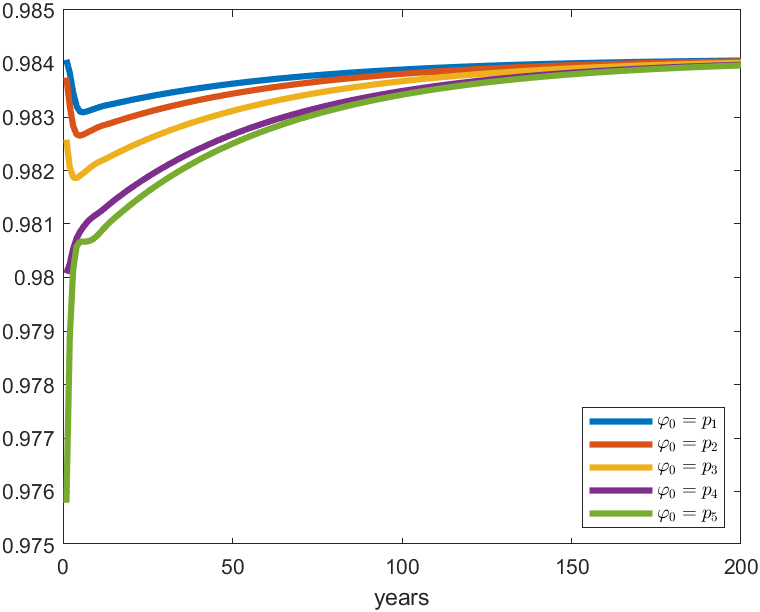
\includegraphics[width=0.6\linewidth]{Images/F=0.05/spectral_radius_when_f=0.05}
	\caption{Spectral radius of $T_{w_t}$ when fecundity is $0.05f(x)$}
	\label{fig:spectralradiuswhenf=0.05}
\end{figure}

Since the spectral radii $r(T_{w_t})$ appear to converge to the value $r(T_1)$, where the latter is the growth rate when the biomass is zero, one may wonder if the total population and biomass in fact go to zero. This does appear to be the case:

\begin{figure}[H]
	\centering
	\begin{minipage}{.43\textwidth}
	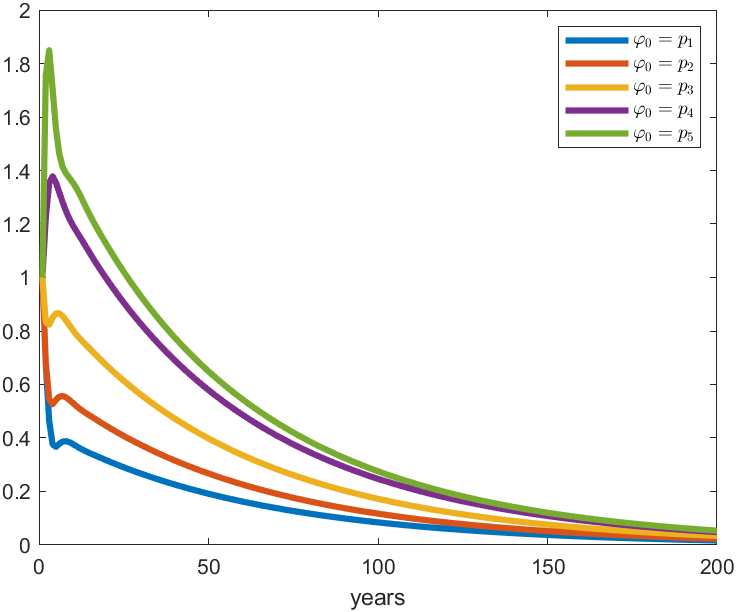
\includegraphics[width=\linewidth]{Images/F=0.05/total_pop_when_f=0.05}
	\caption{Total population}
	\label{fig:totalpopwhenf=0.05}
	\end{minipage} \quad 
	\centering
	\begin{minipage}{.43\textwidth}
	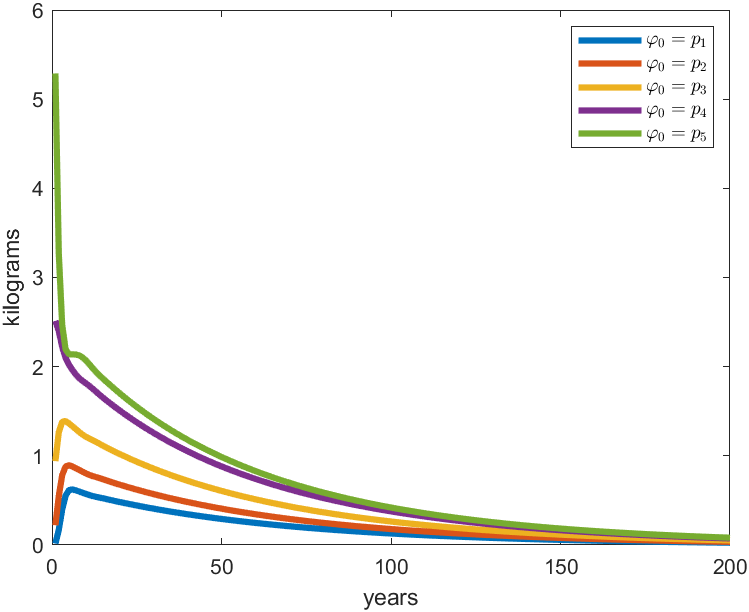
\includegraphics[width=\linewidth]{Images/F=0.05/total_biomass_when_f=0.05}
	\caption{Total biomass}
	\label{fig:totalbiomasswhenf=0.05}
	\end{minipage}
\end{figure}

Even though the population vectors $\varphi_t$ approach 0, the normalized vectors $\varphi_t / || \varphi_t||$ converge to a stable stage distribution, which is the leading eigenvector of $T_1$. Note that $T_1$ is the same as the linear operator with kernel \ref{eqn:kernel}, which incorporates no density-dependence in somatic growth. Hence, this is the distribution we compare later distributions with in order to determine whether a population is dominated by small individuals:

\begin{figure}[H]
	\centering
	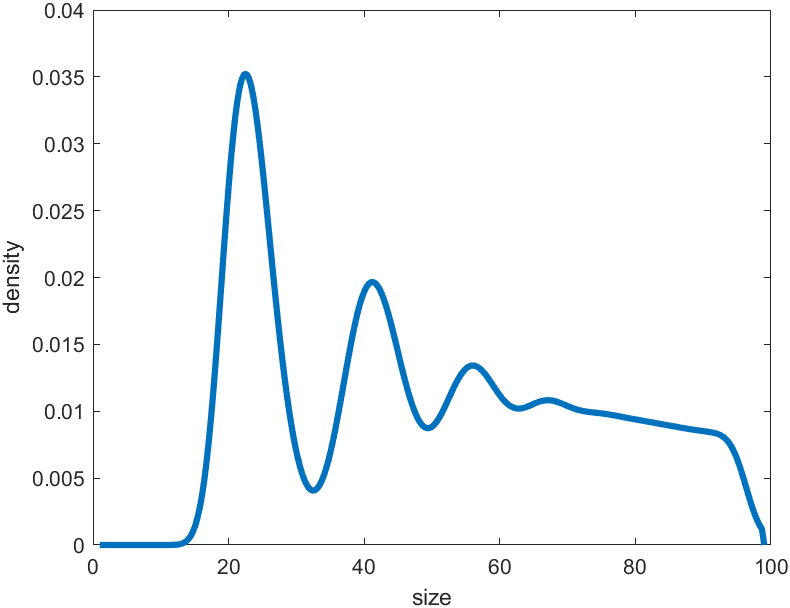
\includegraphics[width=0.6\linewidth]{Images/F=0.05/ssd_when_f=0.05}
	\caption{Stable stage distribution, also the leading eigenvector of $T_1$}
	\label{fig:ssdwhenf=0.05}
\end{figure}

Note that the sharp decrease near the upper size limit $U$ is a result of the difficulty in approximating the kernel near $(U,U)$, since the kernel is unbounded in any neighborhood of that point.

\subsection{Simulations for the Fecundity Function $f(x)$} \label{subsec:f(x)}

For the kernel with fecundity function $f(x)$, we found that $r(T_{0.001}) < 1 < r(T_1)$, a situation similar to conclusion (4) of Theorem \ref{thm:finitedimtheorem}. That result states that the matrix system \eqref{eqn:system} approaches a nonzero equilibrium population. In other words, $r(A_{w_t}) \to 1$, which also appears to happen in the case of the IPM system:

\begin{figure}[H]
	\centering
	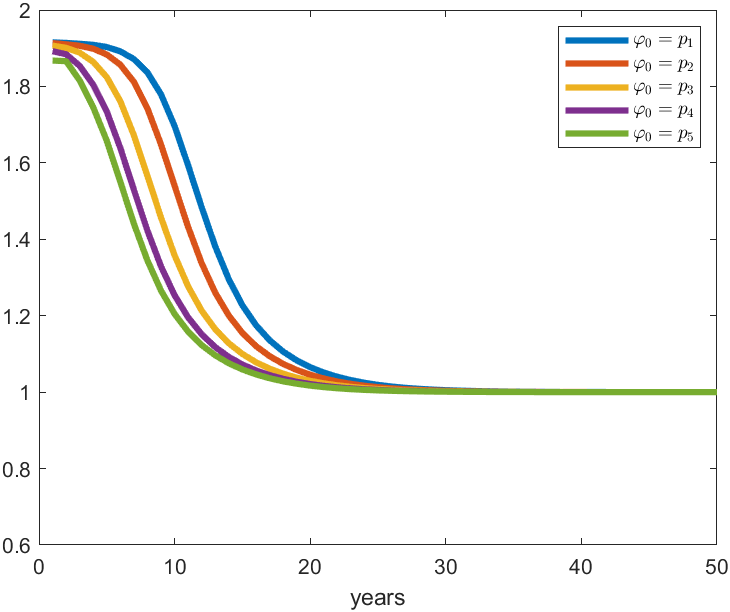
\includegraphics[width=0.6\linewidth]{Images/F=1/spectral_radius_when_f=1}
	\caption{Spectral radius of $T_{w_t}$ when fecundity is $f(x)$}
	\label{fig:spectralradiuswhenf=1}
\end{figure}

Additionally, the total population and biomass approach positive values:

\begin{figure}[H]
	\centering
	\begin{minipage}{.43\textwidth}
		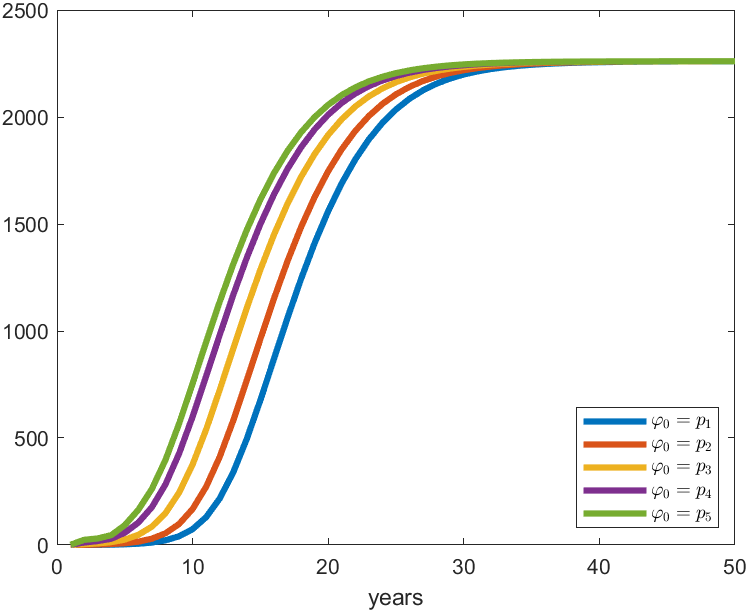
\includegraphics[width=\linewidth]{Images/F=1/total_pop_when_f=1}
		\caption{Total population}
		\label{fig:totalpopwhenf=1}
	\end{minipage} \quad 
	\centering
	\begin{minipage}{.43\textwidth}
		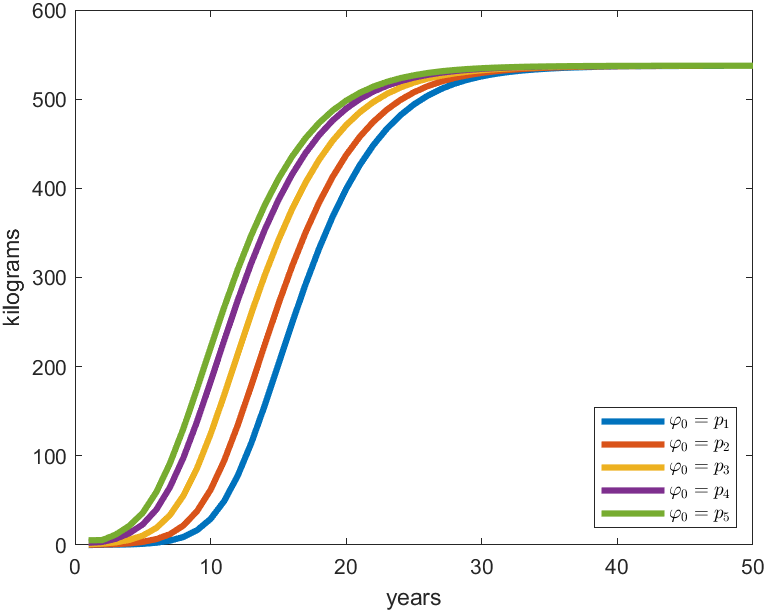
\includegraphics[width=\linewidth]{Images/F=1/total_biomass_when_f=1}
		\caption{Total biomass}
		\label{fig:totalbiomasswhenf=1}
	\end{minipage}
\end{figure}

In this case, the population vector converges to an equilibrium distribution, which is also the leading eigenvector of $T_{w(B^*)}$, where $B^*$ is the equilibrium biomass indicated in Figure \ref{fig:totalbiomasswhenf=1}:

\begin{figure}[H]
	\centering
	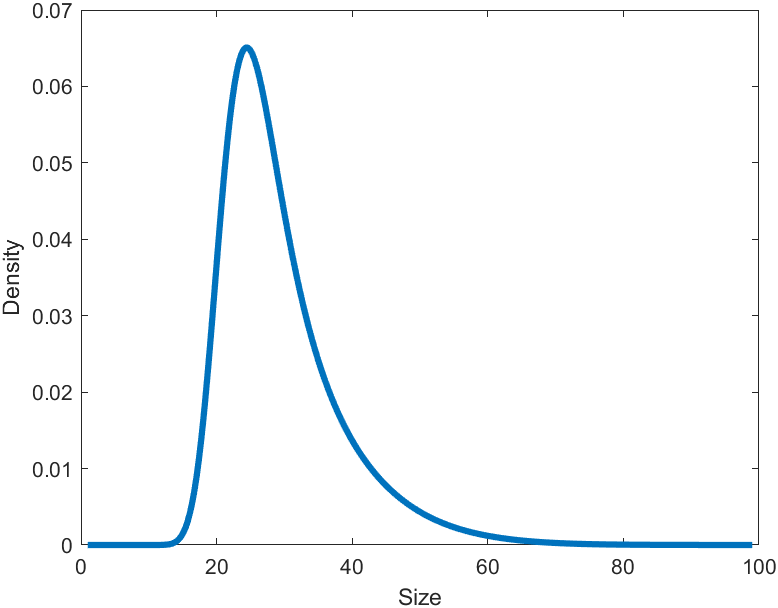
\includegraphics[width=0.6\linewidth]{Images/F=1/ssd_when_f=1}
	\caption{Stable stage distribution, also the leading eigenvector of $T_{w(B^*)}$}
	\label{fig:ssdwhenf=1}
\end{figure}

Note the contrast between Figures \ref{fig:ssdwhenf=0.05} and \ref{fig:ssdwhenf=1}; when the total biomass approaches a positive value, the stable stage distribution shows inhibited growth. The distribution in Figure \ref{fig:ssdwhenf=1} is more concentrated in small sizes, and individuals do not grow much past the spike of the offspring distribution.

\subsection{Simluations for the Fecundity Function $1000f(x)$} \label{subsec:1000f(x)}

Conclusion (3) of Theorem \ref{thm:finitedimtheorem} gives a sufficient condition for the population to grow without bound, namely when $r(A_0) >1$. In order to avoid division by zero in our model, the lowest value $w_t$ can attain is $0.001$, so we investigated whether the population in the IPM model goes to infinity when $r(T_{0.001}) > 1$. This occurs for a fecundity function given by $1000f(x)$, but even with this dramatic increase, our estimate for $r(T_{0.001})$ was only barely greater than 1. In this case, we expected $r(T_{w_t}) \to r(T_{0.001}) > 1$, which does appear to be the case. In the following plot, we included a dotted line to show that the spectral radii stay bounded away from (and above) 1:

\begin{figure}[H]
	\centering
	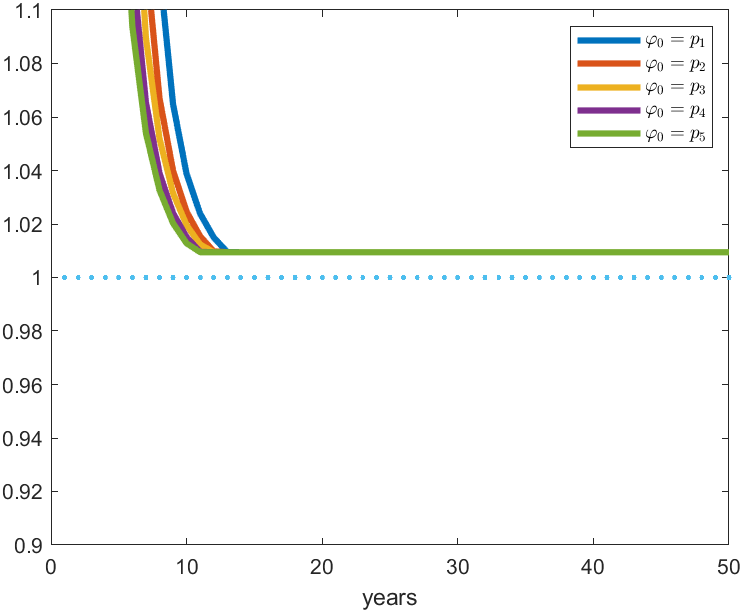
\includegraphics[width=0.6\linewidth]{Images/F=1000/spectral_radius_when_f=1000}
	\caption{Spectral radius of $T_{w_t}$ when fecundity is $1000f(x)$}
	\label{fig:spectralradiuswhenf=1000}
\end{figure}

As expected, the total population and biomass increase without bound:

\begin{figure}[H]
	\centering
	\begin{minipage}{.43\textwidth}
		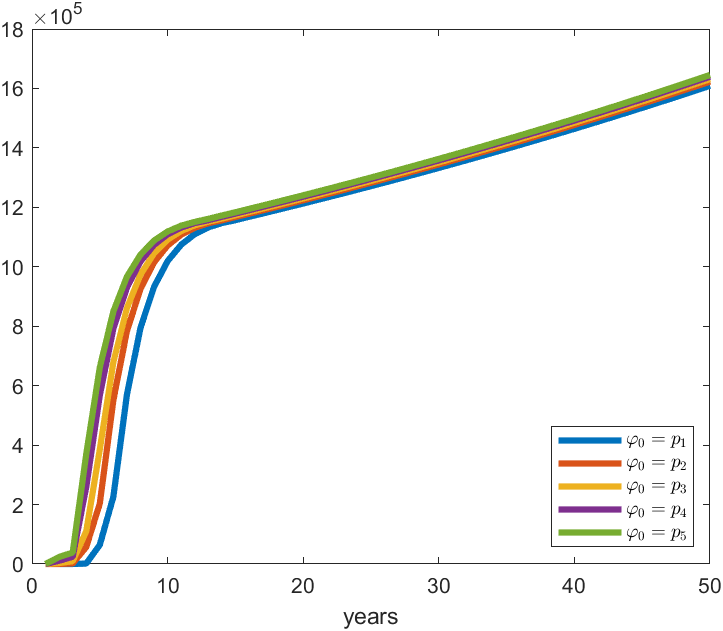
\includegraphics[width=\linewidth]{Images/F=1000/total_pop_when_f=1000}
		\caption{Total population}
		\label{fig:totalpopwhenf=1000}
	\end{minipage} \quad 
	\centering
	\begin{minipage}{.43\textwidth}
		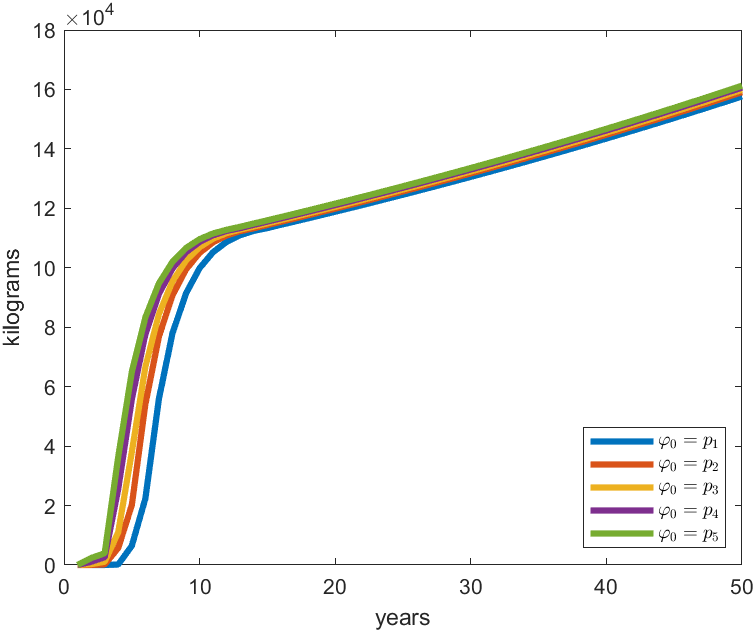
\includegraphics[width=\linewidth]{Images/F=1000/total_biomass_when_f=1000}
		\caption{Total biomass}
		\label{fig:totalbiomasswhenf=1000}
	\end{minipage}
\end{figure}

Since the biomass increases without bound, the values $w_t$ eventually attain the lower bound $0.001$, and the population increases at a rate given by $r(T_{0.001})$. Hence, the population growth is eventually modeled by a linear function, and the stable stage distribution is the leading eigenvector of $T_{0.001}$:

\begin{figure}[H]
	\centering
	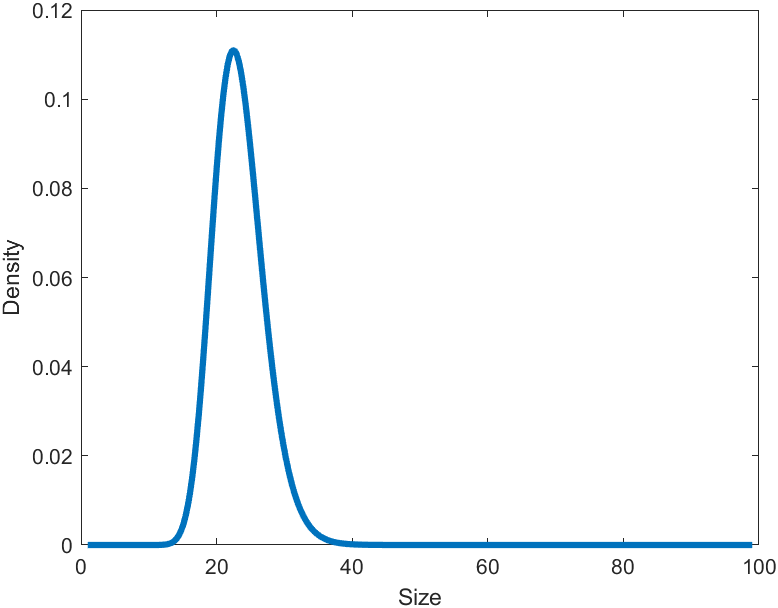
\includegraphics[width=0.6\linewidth]{Images/F=1000/ssd_when_f=1000}
	\caption{Stable stage distribution}
	\label{fig:ssdwhenf=1000}
\end{figure}

Note that Figure \ref{fig:ssdwhenf=1000} indicates a more extreme case of inhibited growth than in Figure \ref{fig:ssdwhenf=1}, since the biomass continues to increase (though $w_t$ attains its lower bound of 0.001).













